\chapter{Methodology for mapping NAPLAN scale scores to \mbox{equivalent} year levels} \label{chap3}

\section{Introduction}


The NAPLAN scale is designed to be independent of year level -- a student should receive the same score on average regardless of whether they take a test normally administered to \mbox{Year 3}, \mbox{Year 5}, \mbox{Year 7} or \mbox{Year 9} students.\footnote{A student's NAPLAN scale score will generally be a more precise estimate of their true skill level when they are administered an age-appropriate test. Giving a typical \mbox{Year 3} student a test meant for \mbox{Year 9} students is likely to produce a NAPLAN scale score with a large standard error.} This property makes it possible to compare students in different test-taking year levels. For example, a \mbox{Year 5} student is predicted to be reading above the typical \mbox{Year 7} level if they score higher than the typical \mbox{Year 7} student in NAPLAN reading. But because NAPLAN tests are only administered to students in four different year levels, it is not possible to compare students to those outside these year levels without further assumptions.

\textit{Widening gaps} presents a new framework from which to interpret NAPLAN results. NAPLAN scale scores are mapped onto a new measure, \textit{equivalent year levels}. The NAPLAN scale score corresponding to the equivalent year level 4, for example, is the median score expected from students if they took an age-appropriate NAPLAN test when they were in \mbox{Year 4}.\footnote{To be precise, in May of the year they were in \mbox{Year 4}, as this is when the NAPLAN test is taken.}  

This appendix outlines the theoretical framework for mapping NAPLAN scale scores onto equivalent year levels and the methodology and assumptions used to estimate this relationship.

\section{Theoretical framework for mapping} \label{sec:theoretical}

Let $X_{j}$ ($X_{j} \in \mathbb{R}$) be a random variable denoting student skill level (as estimated by NAPLAN scale scores) in domain ${j}$ ($j = $ reading, numeracy), and $Y$ be a variable denoting schooling year level, continuous over the range of schooling years, $\left(y_{min},y_{max}\right)$.\footnote{Lower case letters are used to denote realisations of these random variables. This report's analysis focuses on reading and numeracy only, but it would be possible to apply the same analysis to the other assessment domains.}

We assume that median student skill level increases monotonically as students progress through school. We define a function $f_{j}(Y)$ as the median of $X_{j}$ conditional on $Y$:
\newcommand\numberthis{\addtocounter{equation}{1}\tag{\theequation}}
\begin{align*}
 f_{j}(Y) &= Q_{50}\left[X_{j} \mid Y\right]  \\ 
 y_1 < y_2 &\implies f_{j}(y_{1}) < f_{j}(y_{2}) \numberthis\label{eq:median} \\ 
 f_{j}(Y) &\in \left[f_{j}(y_{\min}),f_{j}(y_{\max})\right] 
\end{align*}
That is, $f_{j}(Y)$ is the median NAPLAN scale score in domain ${j}$ of students taking a NAPLAN test in year level $Y$. For every schooling level there is a corresponding median NAPLAN scale score (for each domain). We also assume that $f_{j}(Y)$ is continuous and monotonically increasing -- at the population level, median student skill level increases steadily over time.\footnote{For example, if NAPLAN tests were taken every month, we would expect the median score to improve with every test. This may not hold for individual students, but should hold at the population level.}

\newpage
Following this, we propose that a given NAPLAN scale score corresponds to a median schooling year -- the point in time in the median student's path of progress (in terms of year level and months) at which their skill level is equal to that score. We define this schooling year as an \textit{equivalent year level}, denoted as $Y^{*}$:
\begin{equation} Y^{*} = f_{j}^{-1}\left(X_{j}\right) 
\end{equation}
All NAPLAN scale scores in the range $\left[f_{j}(y_{min}),f_{j}(y_{max})\right]$ therefore correspond to an \textit{equivalent year level}.

\section{Estimating equivalent year levels}

This methodology aims to estimate $f_{j}(Y)$ for reading and numeracy for a range of different year levels, $Y = 1,2,...,12$, then interpolate over these points to construct a smooth curve. If the NAPLAN tests were administered to students in every year level from Year 1 to \mbox{Year 12}, we could estimate $f_{j}(Y)$ as the sample median from each of these year levels.\footnote{This is a useful way of thinking about what equivalent year levels are trying to measure. But it is important to note that the interpretation of equivalent year levels 11 and 12 estimated with the available data could be very different to those estimated with data on \mbox{Year 11} and \mbox{Year 12} students, as explained in \Vref{box:eyl}.} But with the tests only administered in four year levels, we must make further assumptions to estimate $f_{j}(Y)$.

The report estimates $f_{j}(Y)$ (the median NAPLAN scale scores corresponding to a given year level) using the simulated NAPLAN results (see Section \ref{sec:pv}) of all Australian students in 2014 linked to their 2012 simulated results (where applicable). It is possible to apply this methodology to NAPLAN results in other years, provided linked data are available.

\textbf{Step 1: Estimate the median NAPLAN scale scores at year levels 3, 5, 7, and 9}
\nopagebreak

These are estimated as the sample median scores in those year levels:
\begin{equation} \begin{array}{c}
\widehat{f}_{j}(3) = \tilde{x}_{j,3} \vspace{0.3em}\\ \widehat{f}_{j}(5) = \tilde{x}_{j,5} \vspace{0.3em}\\ \widehat{f}_{j}(7) = \tilde{x}_{j,7} \vspace{0.3em}\\
\widehat{f}_{j}(9) = \tilde{x}_{j,9}
\end{array} \end{equation}
where $\tilde{x}_{j,y}$ is the sample median NAPLAN scale score in year level $y$.\footnote{For Years 3, 5, and 7, we estimated the corresponding NAPLAN scale score, $\widehat{f}_{j}(Y)$, as the average of the medians in 2012 and 2014.}

\vspace{9pt}
\textbf{Step 2: Interpolate between \mbox{Year 3} and \mbox{Year 9}}
\nopagebreak

Using a third-order polynomial, fit a smooth curve through the four data points, ($[Y,\widehat{f}_{j}(Y)], Y = 3,5,7,9$), to estimate $f_{j}(Y)$ between \mbox{Year 3} and \mbox{Year 9}, as shown in \Cref{fig:interpolation}.

\begin{figure}[H]
 \captionwithunits{A third-order polynomial is used to interpolate between \mbox{Year 3} and \mbox{Year 9}}{Estimated median NAPLAN scale score, $\widehat{f}_{j}(Y)$, numeracy, Australia}
 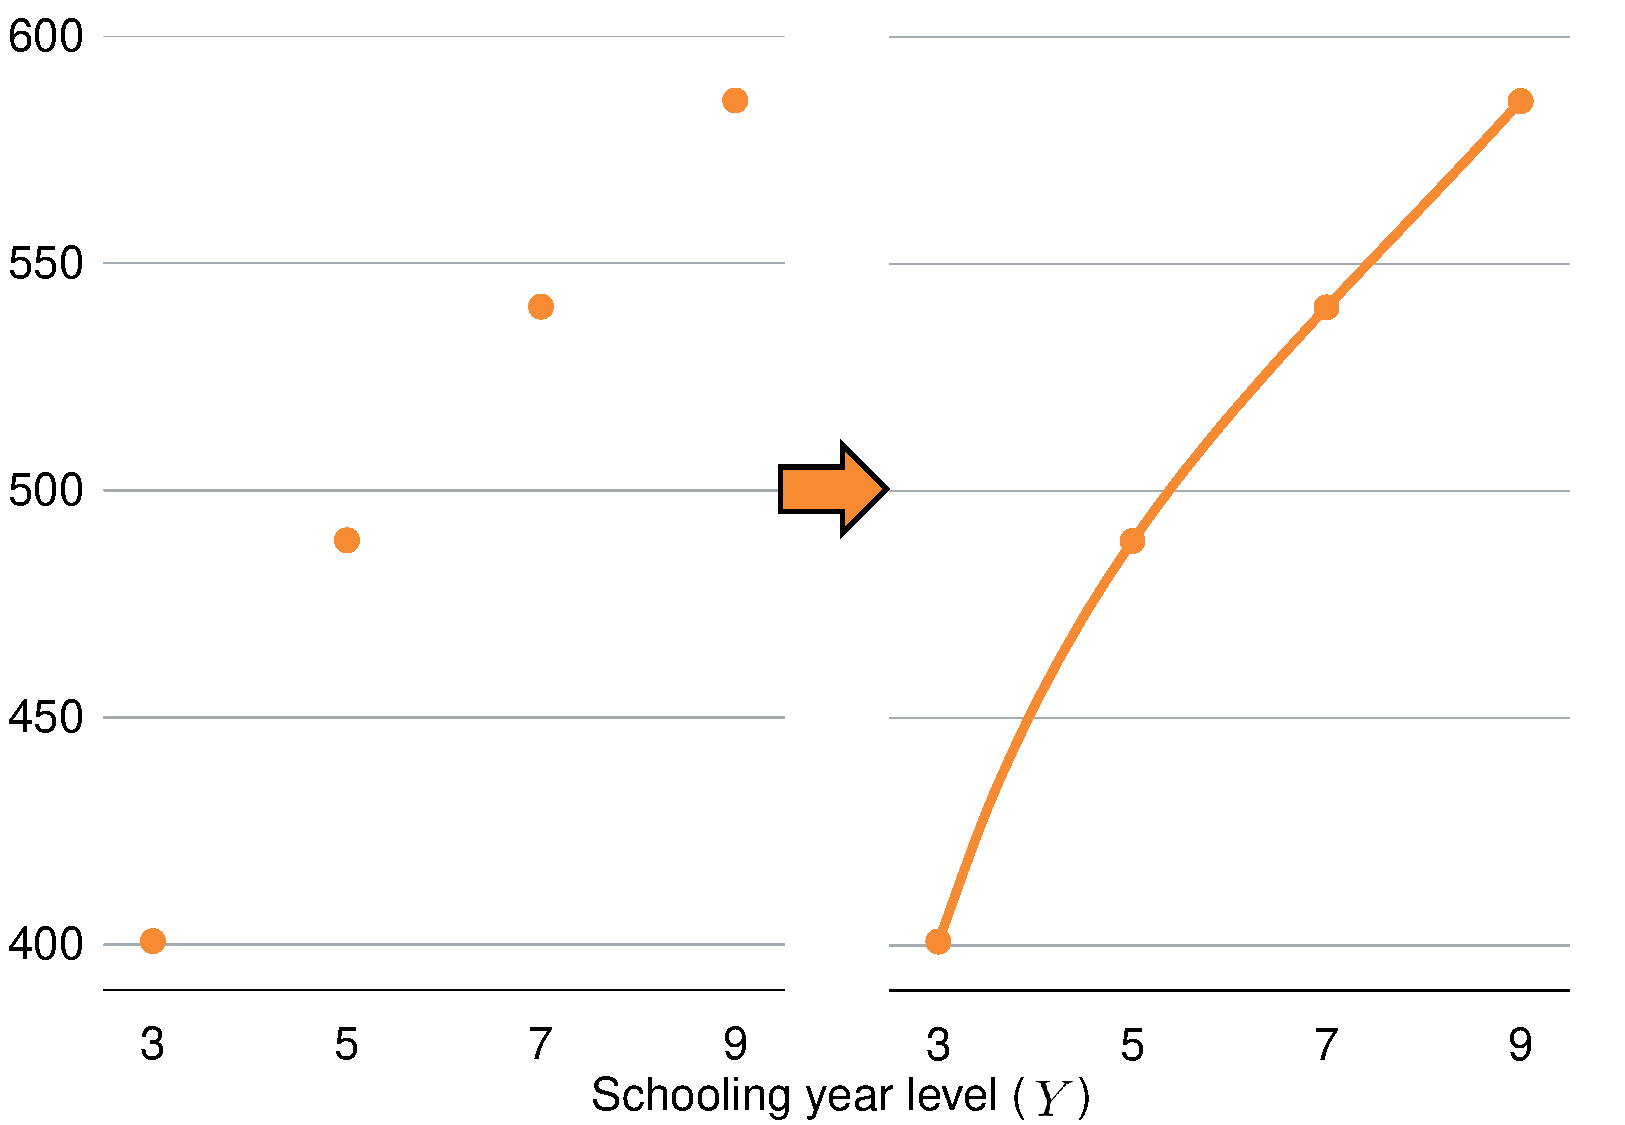
\includegraphics[width=\columnwidth]{atlas/Interpolation.pdf}\label{fig:interpolation}

\source{Grattan analysis of \textcite{acara2014}.}
\end{figure}
\vspace{-6pt}

\textbf{Step 3: Estimate the median gain score for Years 3 to 5 and Years 7 to 9 conditional on prior score} 
\nopagebreak

To estimate $f_{j}(Y)$ above \mbox{Year 9} and below \mbox{Year 3}, we denote a function, $g_{j,Y}\left(X_{j,Y-2} \right)$, equal to the median gain score conditional on year level and a student's NAPLAN scale score from two years earlier:
\begin{equation}
g_{j,Y}\left(X_{j,Y-2} \right) = Q_{50}\left[X_{j,Y}-X_{j,Y-2} | Y, X_{j,Y-2} \right] \label{eq:med_gain}
\end{equation}
where $X_{j,Y}$ denotes NAPLAN scale score in domain $j$ in school year $Y$. For students that scored $x_{j,3}$ in \mbox{Year 3} reading, for example, $g_{j,5}(x_{j,3})$ is the median gain score these students will make to \mbox{Year 5}.\footnote{The function $g_{j,Y}$ can only be empirically estimated for $Y=5$, $7$ and $9$, corresponding to gain scores from Years 3 to 5, Years 5 to 7, and Years 7 to 9 respectively.}   

From \cref{eq:med_gain,eq:median}, it follows that:
\begin{equation} 
g_{j,Y}\left[f_{j}(Y-2)\right] = f_{j}(Y) - f_{j}(Y-2) \label{eq:gf}
\end{equation}
That is, the difference between the median scores two years apart is equal to the median gain made from the same starting score.

To estimate $g_{j,Y}$ for $Y=5$ and $Y=9$ first requires parameterising the functions. We allow for non-linearity in $g_{j,Y}$ by using restricted cubic regression splines, meaning that $g_{j,Y}$ can be written as a linear function:
\begin{equation} \begin{array}{c}
g_{j,Y}(X_{j,Y-2}) = \beta_{0} + \beta_{1}X_{j,Y-2} + \beta_{2}S_{2}(X_{j,Y-2}) \vspace{0.3em}\\
+ \beta_{3}S_{3}(X_{j,Y-2}) + \beta_{4}S_{4}(X_{j,Y-2}) \label{eq:g_jY}
\end{array} \end{equation}
where $S_{2},S_{3}$ and $S_{4}$ are functions that create spline variables.\footnote{More spline variables can be included, if desired.} Alternatively, this function could be specified with quadratic or higher order polynomial terms.

Given $g_{j,Y}$ represents a conditional median gain score, \cref{eq:g_jY} can be thought of as a quantile regression model at the median. This can be estimated using least absolute deviations.\footnote{It is only necessary to estimate $g_{j,5}$ for $x_{j,3}\leq \widehat{f}_{j}(3)$ and $g_{j,9}$ for $x_{j,7} \geq \widehat{f}_{j}(7)$.}

\Cref{fig:g579} plots the estimated functions, $\widehat{g}_{j,y}\left(x_{j,y-2}\right)$, for $y=5,7$ and $9$ for both reading and numeracy. Predicted median NAPLAN gain scores are much higher for lower prior scores, but year level does not have a large effect on gain scores once prior scores are controlled for. For instance, when evaluated at the NAPLAN score for equivalent year level 3, $\widehat{f}_{j}\left(3\right)$, the functions $\widehat{g}_{j,5}$ and $\widehat{g}_{j,7}$ are extremely close for reading, and similar for numeracy. Similarly, when evaluated at equivalent year level 7, $\widehat{f}_{j}\left(7\right)$, the functions $\widehat{g}_{j,9}$ and $\widehat{g}_{j,7}$ are very close for both reading and numeracy. That is, expected NAPLAN gain from a given starting point is similar for students that are two year levels apart.

\begin{figure}[t]
 \captionwithunits{The estimated median gain score is strongly related to prior score, but only weakly related to year level}{Two-year median NAPLAN gain score, $\widehat{g}_{j,y}(x_{j,y-2})$, Australia}
 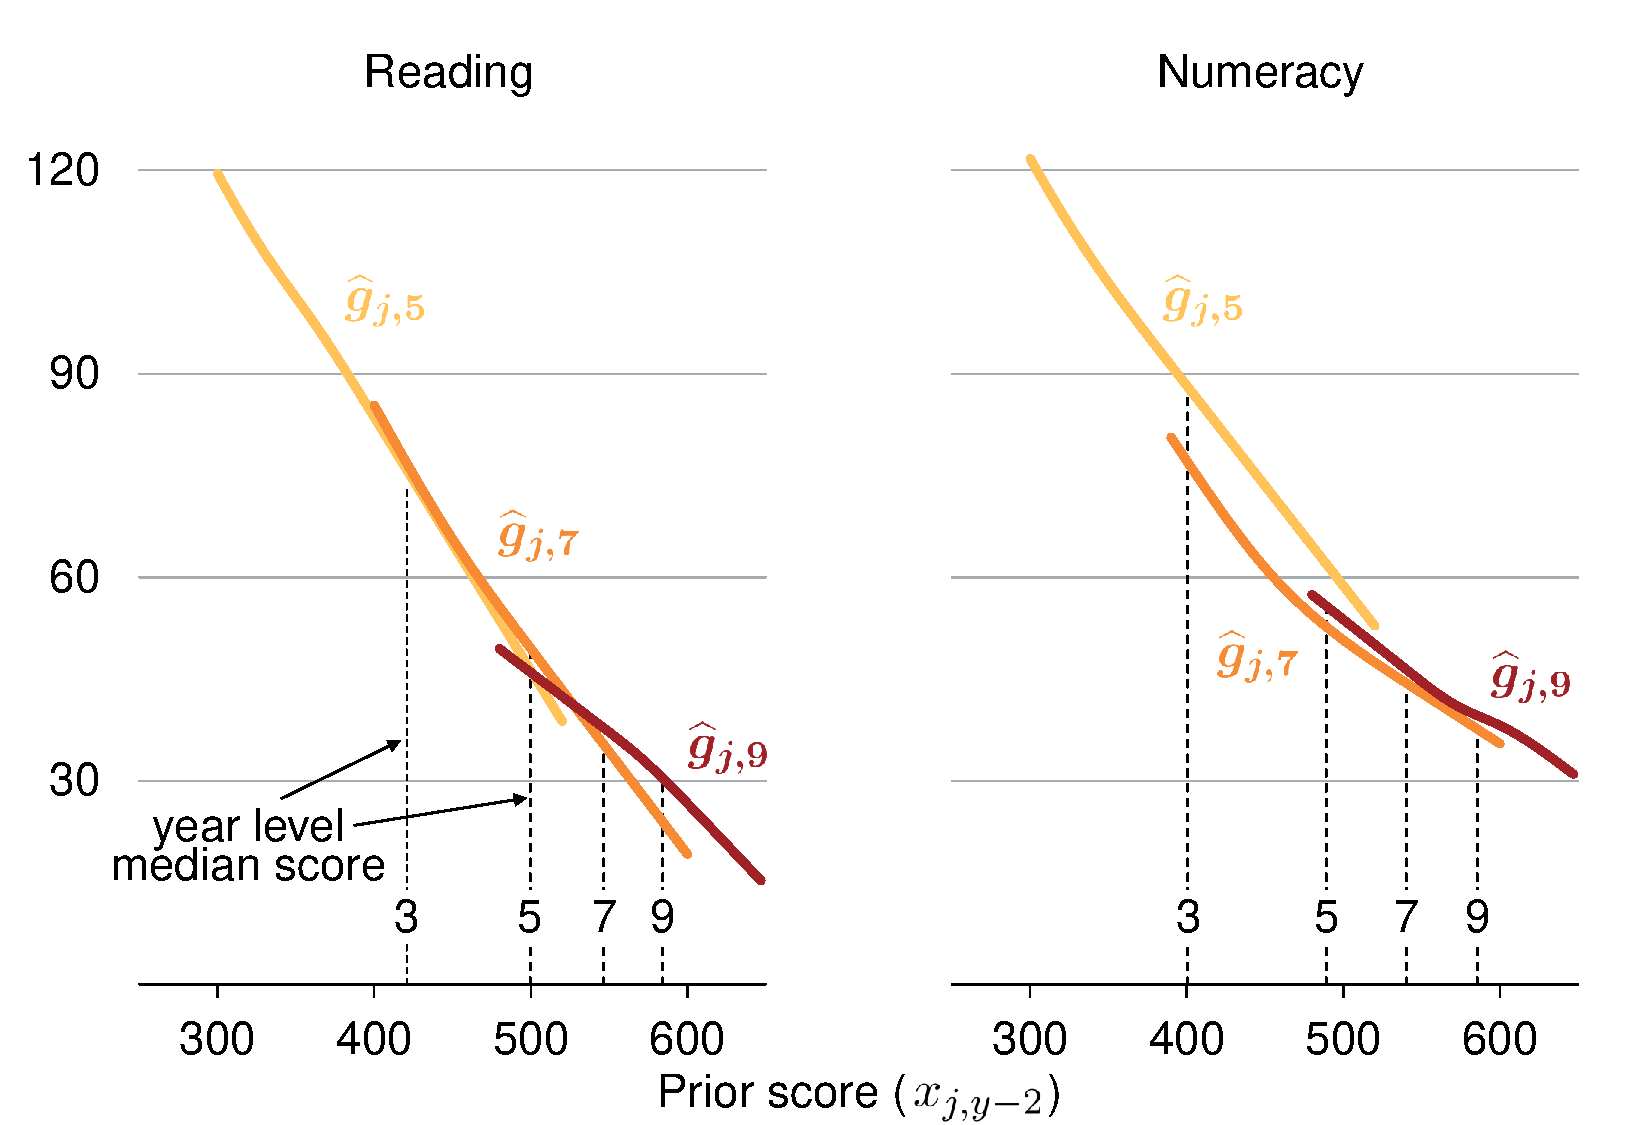
\includegraphics[width=\columnwidth]{atlas/G579.pdf}\label{fig:g579}

\source{Grattan analysis of \textcite{acara2014}.}
\end{figure}

Setting $Y=10$ and re-arranging \cref{eq:gf} gives:
\begin{equation}
f_{j}\left(10\right) = f_{j}\left(8\right) + g_{j,10}\left[f_{j}\left(8\right)\right]
\end{equation}
The point $f_{j}\left(8\right)$ was estimated in Step 2, but it is not possible to estimate $g_{j,10}$ without NAPLAN data for \mbox{Year 10} students (linked to Year 8 results). But given that year level has little effect on gain scores once prior scores are controlled for, we can assume:
\begin{equation}
g_{j,10}\left[f_{j}\left(8\right)\right] \approx g_{j,9}\left[f_{j}\left(8\right)\right] \label{eq:g9g10}
\end{equation}
That is, a student in Year 8 performing at the median Year 8 level will make a similar gain over two years as a \mbox{Year 7} student performing at the median Year 8 level.

It is necessary to make a stronger assumption to estimate $f_{j}\left(11\right)$: 
\begin{equation}
g_{j,11}\left[f_{j}\left(9\right)\right] \approx g_{j,9}\left[f_{j}\left(9\right)\right] \label{eq:g10g11}
\end{equation}
That is, we assume a student in \mbox{Year 9} performing at the median \mbox{Year 9} level will make a similar gain over two years as a \mbox{Year 7} student performing at the median \mbox{Year 9} level.

Similarly, we can use our estimate of $g_{j,5}$ as a proxy for $g_{j,4}$ by assuming:
\begin{equation}
g_{j,4}\left[f_{j}\left(2\right)\right] \approx g_{j,5}\left[f_{j}\left(2\right)\right] \label{eq:g4g5}
\end{equation}
That is, a \mbox{Year 2} student performing at the median \mbox{Year 2} level is assumed to make a similar gain over two years as a \mbox{Year 3} student performing at the median \mbox{Year 2} level.

\vspace{9pt}
\textbf{Step 4: Estimate the median NAPLAN scale scores for year levels 10 and 11}
\nopagebreak

Using the assumptions made in \cref{eq:g9g10} and \cref{eq:g10g11}, $f_{j}(10)$ and $f_{j}(11)$ are estimated using the following:
\begin{equation} \begin{array}{c}
\widehat{f}_{j}\left(10\right) = \widehat{f}_{j}\left(8\right) + \widehat{g}_{j,9}\left[\widehat{f}_{j}\left(8\right)\right] \vspace{0.3em}\\
\widehat{f}_{j}\left(11\right) = \widehat{f}_{j}\left(9\right) + \widehat{g}_{j,9}\left[\widehat{f}_{j}\left(9\right)\right] 
\end{array} \end{equation}
where, for example, $\widehat{f}_{j}(8)$ is the estimated median NAPLAN scale score for Year 8 students, calculated in Step 2, and $\widehat{g}_{j,9}$ is the estimated median NAPLAN gain score function from \mbox{Year 7} to \mbox{Year 9}, calculated in Step 3.

\textbf{Step 5: Estimate the median NAPLAN scale scores for year levels 1.5, 2, and 2.5}
\nopagebreak

Using the assumption made in \cref{eq:g4g5} and its extensions, $f_{j}(1.5),f_{j}(2)$ and $f_{j}(2.5)$ are estimated by solving the following equations for $\widehat{f}_{j}\left(Y\right)$:
\begin{equation} \begin{array}{c}
\widehat{f}_{j}\left(1.5\right) = \widehat{f}_{j}\left(3.5\right) - \widehat{g}_{j,5}\left[\widehat{f}_{j}\left(1.5\right)\right] \vspace{0.3em}\\
\widehat{f}_{j}\left(2\right) = \widehat{f}_{j}\left(4\right) - \widehat{g}_{j,5}\left[\widehat{f}_{j}\left(2\right)\right] \vspace{0.3em}\\
\widehat{f}_{j}\left(2.5\right) = \widehat{f}_{j}\left(4.5\right) - \widehat{g}_{j,5}\left[\widehat{f}_{j}\left(2.5\right)\right]
\end{array} \end{equation}
where, for example, $\widehat{f}_{j}(3.5)$ is the estimated median NAPLAN scale score for \mbox{Year 3} students, six months after the NAPLAN test (November), and $\widehat{g}_{j,5}$ is the estimated median gain score function from \mbox{Year 3} to \mbox{Year 5}, calculated in Step 3. These points are estimated closer together because $f_{j}(Y)$ has a larger gradient for lower values of $Y$.

\vspace{9pt}
\textbf{Step 6: Interpolate over estimated points}
\nopagebreak

Using a range of estimated points for $\left[Y,\widehat{f}_{j}(Y)\right]$ (for example, use $Y$ = 1.5, 2, 2.5, 3, 4, 5, 6, 7, 8, 9, 10, 11), construct a smooth curve for $\widehat{f}_{j}(Y)$ using interpolation.\footnote{Our methodology fits a curve using a regression with restricted cubic splines -- some of the points already estimated for $f_{j}(Y)$ shift slightly as a result.} Using linear extrapolation, this curve is extended so that $y_{min} = 1$ and $y_{max} = 13$ (\mbox{Year 13} is reported as `above \mbox{Year 12}'), although our analysis avoids these extremes as much as possible given the estimates are less robust and standard errors are high.\footnote{See \Vref{box:eyl} for a discussion about the interpretation of equivalent year levels estimated outside the range of \mbox{Year 3} to \mbox{Year 9}. Given the estimated curve, $\widehat{f}_{j}(Y)$ is approximately concave between Year 1.5 and \mbox{Year 11}, we would expect concavity to hold if the curve is extended to Year 1 and \mbox{Year 13}. As such, linear extrapolation is unlikely to underestimate the median scale score for Year 1, \mbox{Year 12}, and \mbox{Year 13} -- this is conservative for estimating the gaps in progress between different groups.}

We now have a curve that estimates the median NAPLAN scale score for each schooling year level: $\widehat{f}_{j}(Y)$. The inverse of this curve is used to estimate the equivalent year level, $Y^{*}$, corresponding to any given NAPLAN scale score, $X_{j}$:
\begin{equation} \widehat{Y}^{*} = \widehat{f}_{j}^{-1}(X_{j}) \end{equation}

\Cref{fig:cyl_inverse} shows this curve for reading and numeracy, both in terms of $\widehat{f}_{j}(Y)$ and in terms of its inverse, $\widehat{f}_{j}^{-1}(X_{j})$. As the chart on the right shows, every NAPLAN score (within the range of the curve) can be mapped to an equivalent year level. A score of 500 in numeracy, for instance, corresponds to an equivalent year level of 5 years and 4 months -- a student at this level can be interpreted as performing four months ahead of the typical (median) \mbox{Year 5} student at the time of the \mbox{Year 5} NAPLAN test.\footnote{Given that NAPLAN is administered in May of each year, another interpretation is to say that this student is performing at the level we would expect of the typical \mbox{Year 5} student in September.}

\begin{figure}[H]
 \captionwithunits{All NAPLAN scale scores in a given range correspond to an equivalent year level}{Median NAPLAN scale score \hspace{3.1em} Equivalent year level ($\widehat{Y}^{*}$)}
 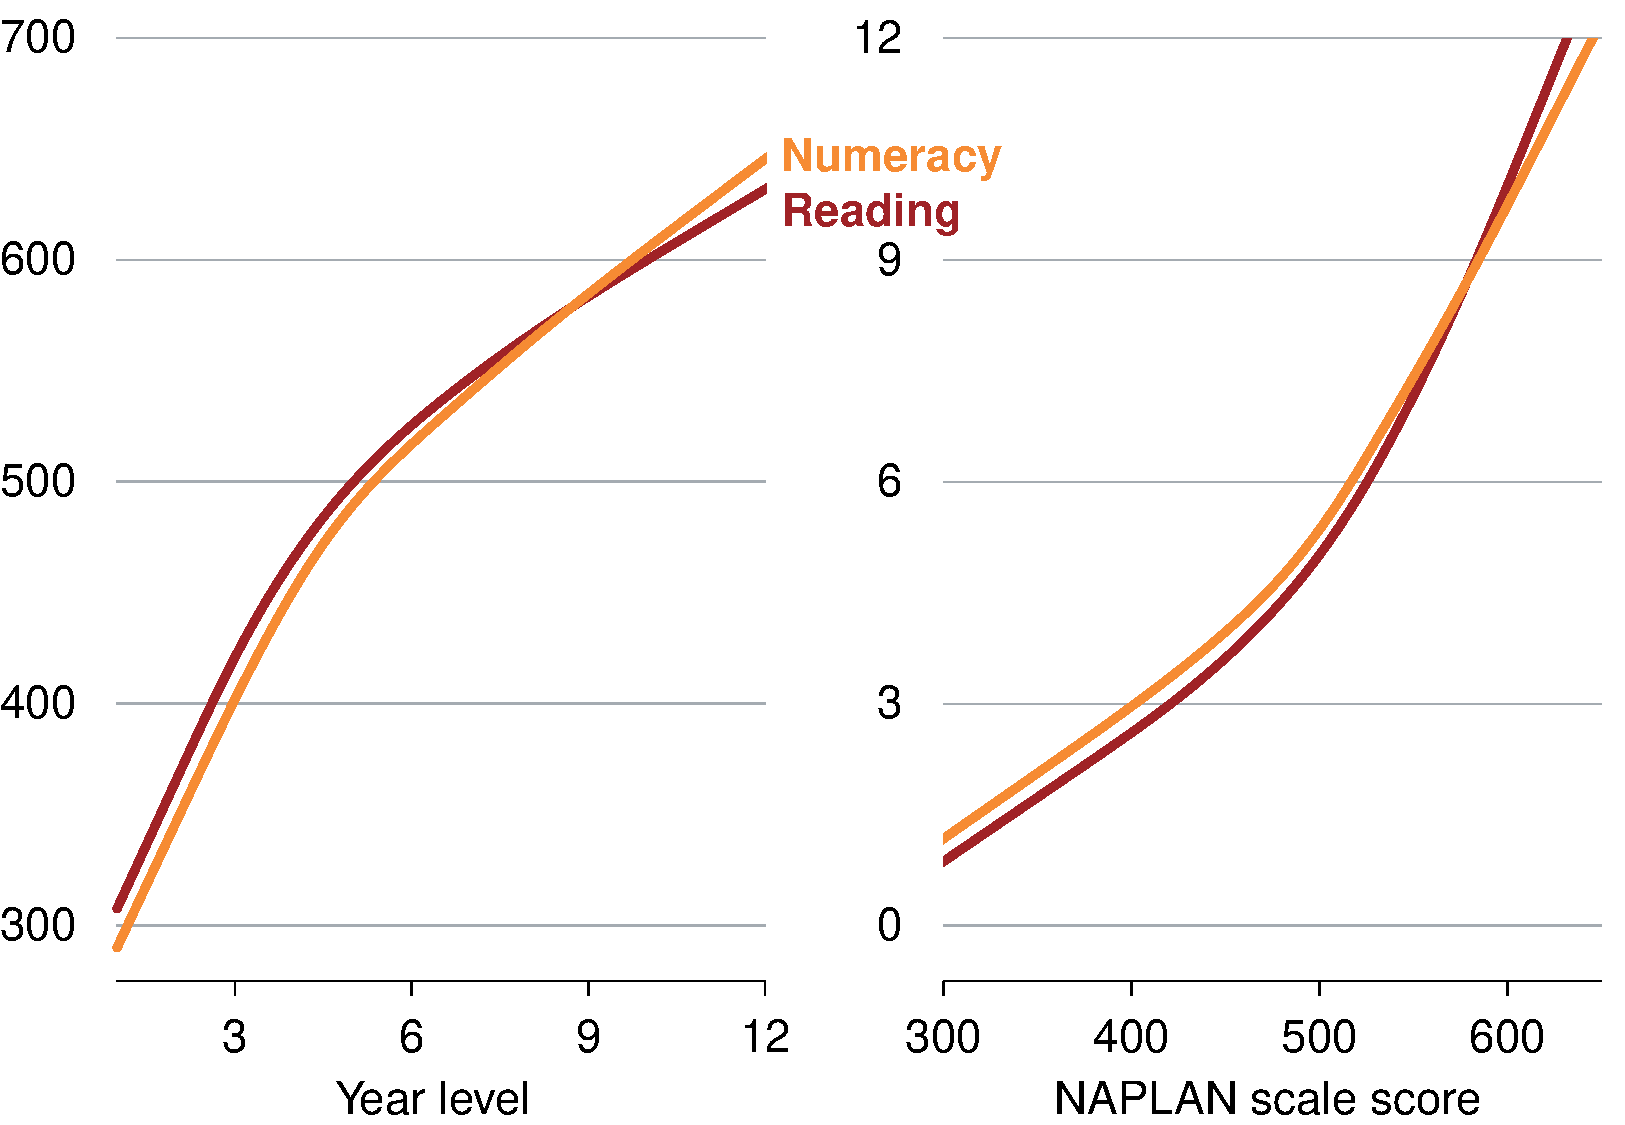
\includegraphics[width=\columnwidth]{atlas/CYL_and_inverse.pdf}\label{fig:cyl_inverse}
\notes{Left chart shows estimated function $\widehat{f}_{j}(Y)$, while right chart shows its inverse, $\widehat{f}_{j}^{-1}(X_{j})$. The left chart can be interpreted as the estimated median NAPLAN scale score for a given year level, whereas the right chart can be interpreted as the estimated equivalent year level for a given NAPLAN scale score.}

\source{Grattan analysis of \textcite{acara2014}.}
\end{figure}
\vspace{-6pt}

\newpage
These curves can be used to compare different cohorts or sub-groups of students in terms of differences in their achievement, and to track student progress relative to the median student. Years of progress is simply calculated as the difference in equivalent year levels between two points in time. If, for example, a student makes 2 years and 6 months of progress over a two-year period, they have made the same amount of progress as the typical (median) student is expected to make over 2 years and 6 months, starting from the same point.

\newpage
\section{Robustness of equivalent year level estimates}

There are a number of questions that may arise in relation to the methodology used to estimate equivalent year levels. For instance:
\begin{itemize}
    \item what is the standard error at different points along the equivalent year level curve?
    \item how accurate are estimates beyond \mbox{Year 3} and \mbox{Year 9}?
    \item how do the estimates change with different assumptions?
    \item are the results robust to the cohort used?
\end{itemize}

It is worth investigating each of these questions in detail to ensure that the methodology and the results are robust.

\subsection{Standard errors around point estimates} \label{sec:se_pe}

There are two sources of error that the standard error accounts for: test measurement error for individuals, and the error associated with a finite sample. But the equivalent year level curve is calculated from a very large sample, meaning that the standard error around estimates of the median is naturally small.\footnote{This assumes that individual measurement error is not systematically biased.}

In reporting, we prefer using confidence intervals to standard errors, since equivalent year levels are asymmetrically distributed around NAPLAN scale scores. We calculate a 99 per cent confidence interval at each point along the curve, $\widehat{f}_{j}(Y)$, between $Y=1$ and $Y=13$. This is based on a bootstrap simulation with 200 replications.\footnote{Each replication uses a different set of random draws. The lower bound at each point is the average of the two lowest simulated points, while the upper bound at each point is the average of the two highest simulated points.}

\newpage
Between \mbox{Year 3} and \mbox{Year 9}, equivalent year levels are estimated with a very narrow confidence interval. As the curve is flatter in \mbox{Year 9} than it is in \mbox{Year 3}, the confidence interval around \mbox{Year 9} is wider. The width of the confidence interval naturally increases below \mbox{Year 3} or above \mbox{Year 9}. For a score of just over 300 in reading (close to equivalent year level 1), the 99 per cent confidence interval around the equivalent year level estimate is about seven months of learning, while for a score of 650 (close to equivalent year level 13), the 99 per cent onfidence interval is eight months.\footnote{In numeracy, the confidence intervals are smaller -- three months at the bottom end, and five months at the top end.} But for scores between 400 and 600, the 99 per cent confidence interval does not exceed two months of learning. These intervals are displayed in  \Cref{fig:cyl_ci,tab:cyl_ci}.

It should be noted that these confidence intervals are calculated under the assumptions in the modelling process. They tell us that the error due to measurement and sample size is likely to be small at most equivalent year levels. They do not tell us whether or not the methodology is appropriate. If we were to account for uncertain assumptions, the intervals would be wider.

\begin{figure}[H]
 \captionwithunits{Confidence intervals are much wider in the extremes}{Estimated 99 per cent confidence interval for equivalent year levels, Australia}
% \vspace{-1.2em}
 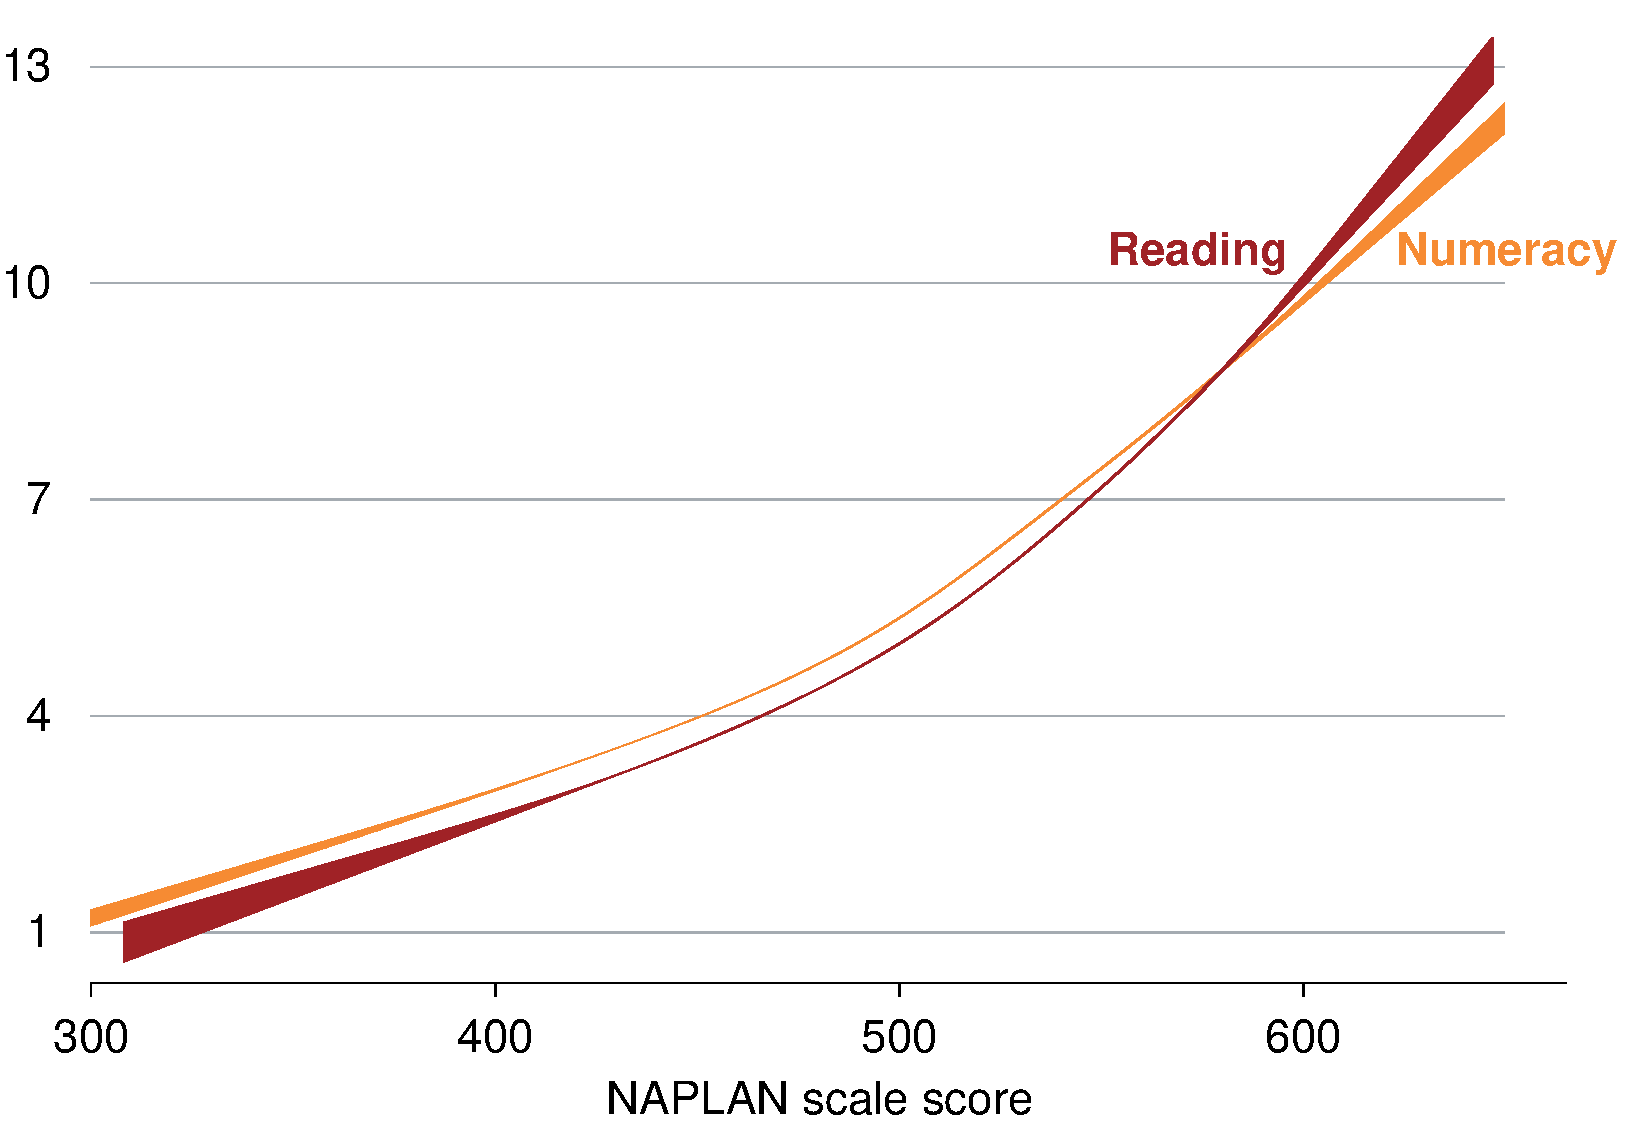
\includegraphics[width=\columnwidth]{atlas/CYL_CI.pdf}\label{fig:cyl_ci}

\source{Grattan analysis of \textcite{acara2014}.}
\end{figure}

\begin{table}[H]
\vspace{-10pt}
  \centering
  \caption{Estimated equivalent year levels with 99 per cent confidence interval, Australia}
  
      \begin{tabular}{lrlrl}

        \multirow{2}[4]{1.5cm}{NAPLAN score}  & \multicolumn{2}{c}{Reading} & \multicolumn{2}{c}{Numeracy} \\
    \cmidrule(lr){2-3} \cmidrule(lr){4-5}
      & $\widehat{Y}^{*}$ & \; Interval & $\widehat{Y}^{*}$ & \; Interval \\ \midrule
    325   & 1.30  & (0.94, 1.42) & 1.62  & (1.55, 1.72) \\
    350   & 1.74  & (1.47, 1.82) & 2.06  & (2.01, 2.14) \\
    375   & 2.17  & (2.00, 2.23) & 2.51  & (2.48, 2.55) \\
    400   & 2.61  & (2.53, 2.64) & 2.97  & (2.95, 2.99) \\
    425   & 3.08  & (3.07, 3.09) & 3.45  & (3.44, 3.46) \\
    450   & 3.62  & (3.60, 3.63) & 3.97  & (3.96, 3.98) \\
    475   & 4.25  & (4.23, 4.25) & 4.58  & (4.57, 4.59) \\
    500   & 5.01  & (4.99, 5.02) & 5.36  & (5.34, 5.37) \\
    525   & 5.98  & (5.97, 6.00) & 6.34  & (6.32, 6.36) \\
    550   & 7.16  & (7.15, 7.19) & 7.42  & (7.40, 7.44) \\
    575   & 8.51  & (8.49, 8.54) & 8.54  & (8.53, 8.58) \\
    600   & 10.00 & (9.95, 10.12) & 9.74  & (9.71, 9.81) \\
    625   & 11.57 & (11.45, 11.89) & 10.98 & (10.89, 11.15) \\
    650   & 13.15 & (12.94, 13.65) & 12.22 & (12.08, 12.50) \\
    \bottomrule
    \end{tabular}%
  \label{tab:cyl_ci}%
\begin{flushleft}\notes{Parentheses show upper and lower bounds of 99 per cent confidence interval for estimated equivalent year levels. This is estimated by a bootstrap simulation with 200 replications. Some estimated equivalent year levels and confidence bounds are below $y_{min}=1$ or above $y_{max}=13$, which shows how wide the intervals are at such points.}

\source{Grattan analysis of \textcite{acara2014}.}\end{flushleft}
\vspace{-6pt}
\end{table}%

\newpage
\subsection{Accuracy of estimates beyond \mbox{Year 3} and \mbox{Year 9}}

Without students taking a NAPLAN test outside of the test-taking years, it is impossible to validate whether our estimates of the median NAPLAN scale score in Years 2, 10, and 11, for instance, reflect how the median student would actually perform in those year levels.\footnote{As discussed in \Vref{box:eyl}, equivalent year level 11 in numeracy may not actually represent the typical \mbox{Year 11} numeracy student, because of curriculum changes and greater student autonomy over subject choices in senior secondary school. The issue is therefore whether equivalent year level 11 is an accurate estimate of where a typical \mbox{Year 9} student would be in two years time if they continued to study numeracy or reading in a similar way.} But it is possible to use a similar methodology to predict the median score in \mbox{Year 3} and \mbox{Year 9} without using data from \mbox{Year 3} and \mbox{Year 9}. This can then be compared to the estimated median NAPLAN scale score for \mbox{Year 3} and \mbox{Year 9} on the full dataset. 

Using data for students in \mbox{Year 7} linked to their \mbox{Year 5} results, \Cref{fig:57} shows that the methodology predicts the median NAPLAN scale score outside these year levels with reasonable accuracy (using the curve based on the full dataset as a benchmark). There is some evidence, however, that predicting the median score for year levels well beyond the available data will lead to inaccuracies.\footnote{For instance, using the Years 5 to 7 data overestimates the median score in \mbox{Year 3} numeracy by about 20 NAPLAN points.}

On the whole, the results using Years 5 to 7 data provide a reasonable estimate of equivalent year levels between 18 and 24 months below \mbox{Year 5}, and up to two years ahead of \mbox{Year 7}. Although it is not possible to test the accuracy of our estimates beyond \mbox{Year 3} and \mbox{Year 9}, these results provide some support for the robustness of the methodology.

\begin{figure}[H]
 \captionwithunits{Data from Years 5 and 7 students provides a reasonable approximation for other year levels}{Estimated median NAPLAN scale score, Australia}
% \vspace{-1.2em}
 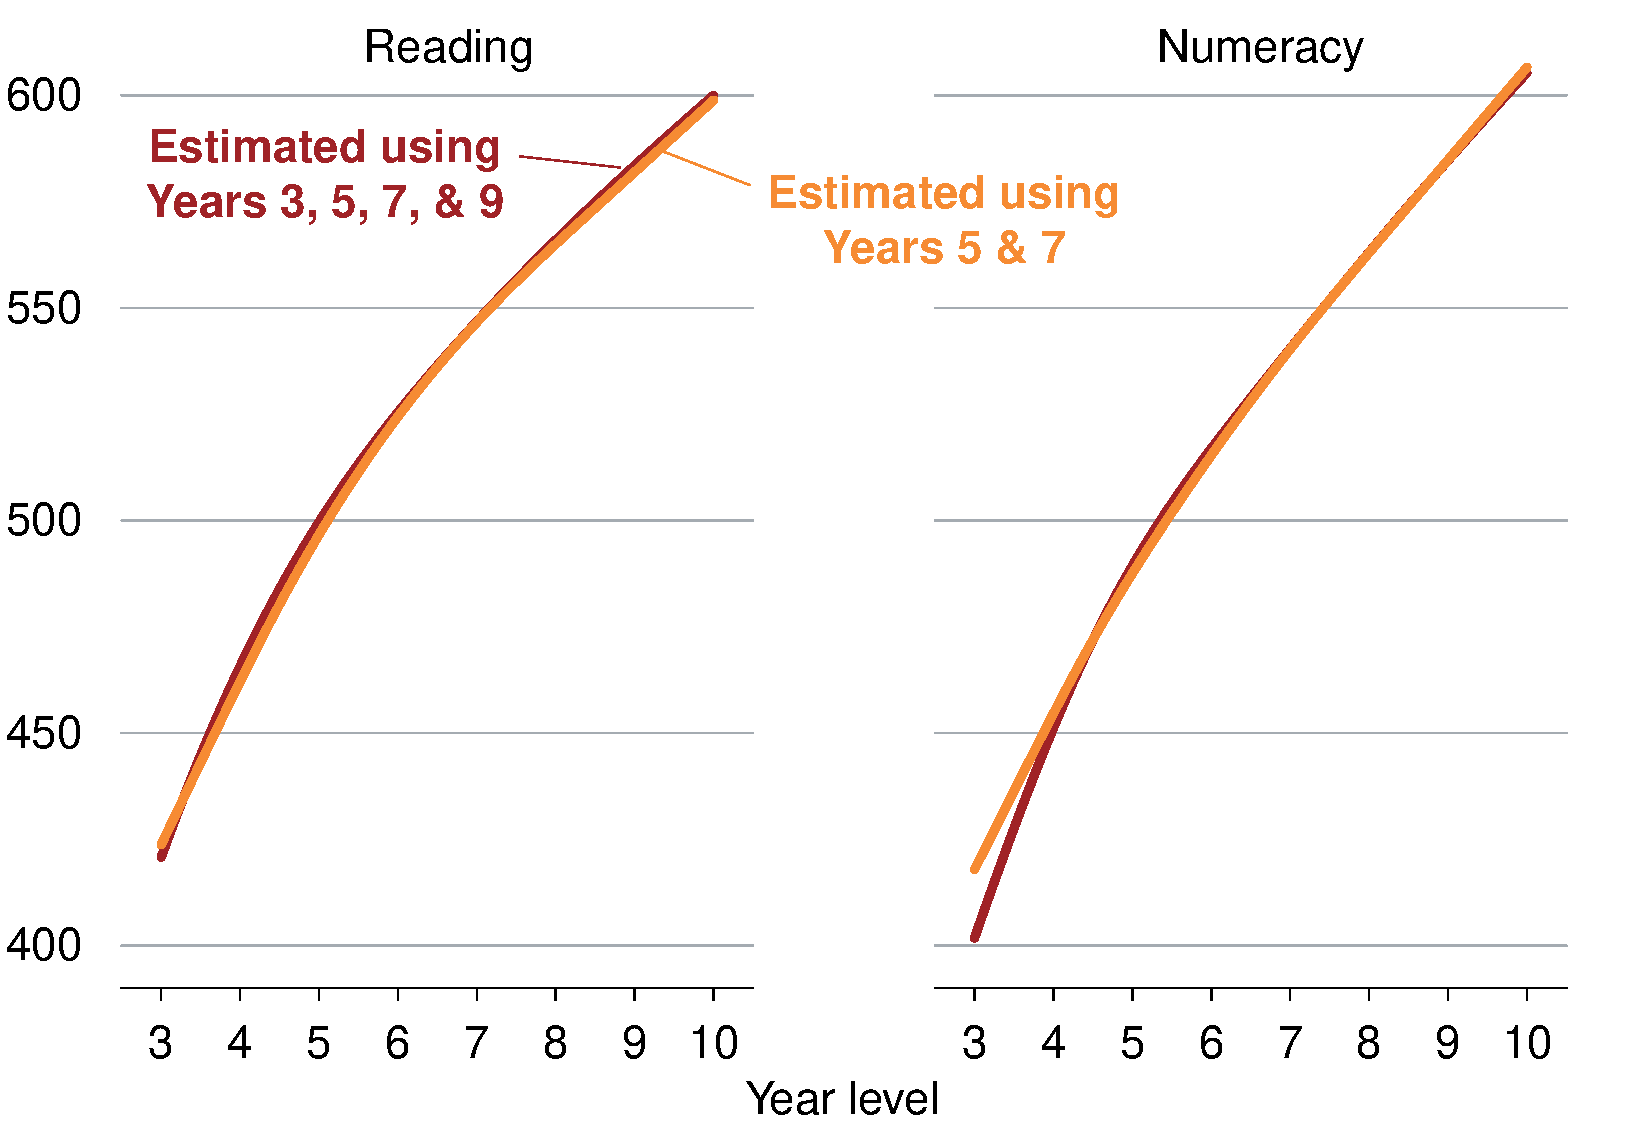
\includegraphics[width=\columnwidth]{atlas/five_seven.pdf}\label{fig:57}

\source{Grattan analysis of \textcite{acara2014}.}
\end{figure}

\newpage
\subsection{How do estimates change with different assumptions?}

\subsubsection{Using a different benchmark student}

Estimates of equivalent year levels are based on the expected path of progress of the median student. Changing the benchmark will not only change the estimated curve, $\widehat{f}_{j}(Y)$, but will also change the definition of the curve.

The most obvious alternative to using the median is to use the mean NAPLAN scale score in each year level. This has a noticeable, but relatively small impact on the shape of the curve, as shown in \Cref{fig:mean_cyl}.\footnote{This curve uses the sample means to estimate $f_{j}(Y)$ for $Y=3,5,7$, and estimates $g_{j,Y}$ via a least squares regression.}

\begin{figure}[t]
 \captionwithunits{Using the mean instead of the median changes the curve slightly}{Estimated median NAPLAN scale score, numeracy, Australia}
% \vspace{-1.2em}
 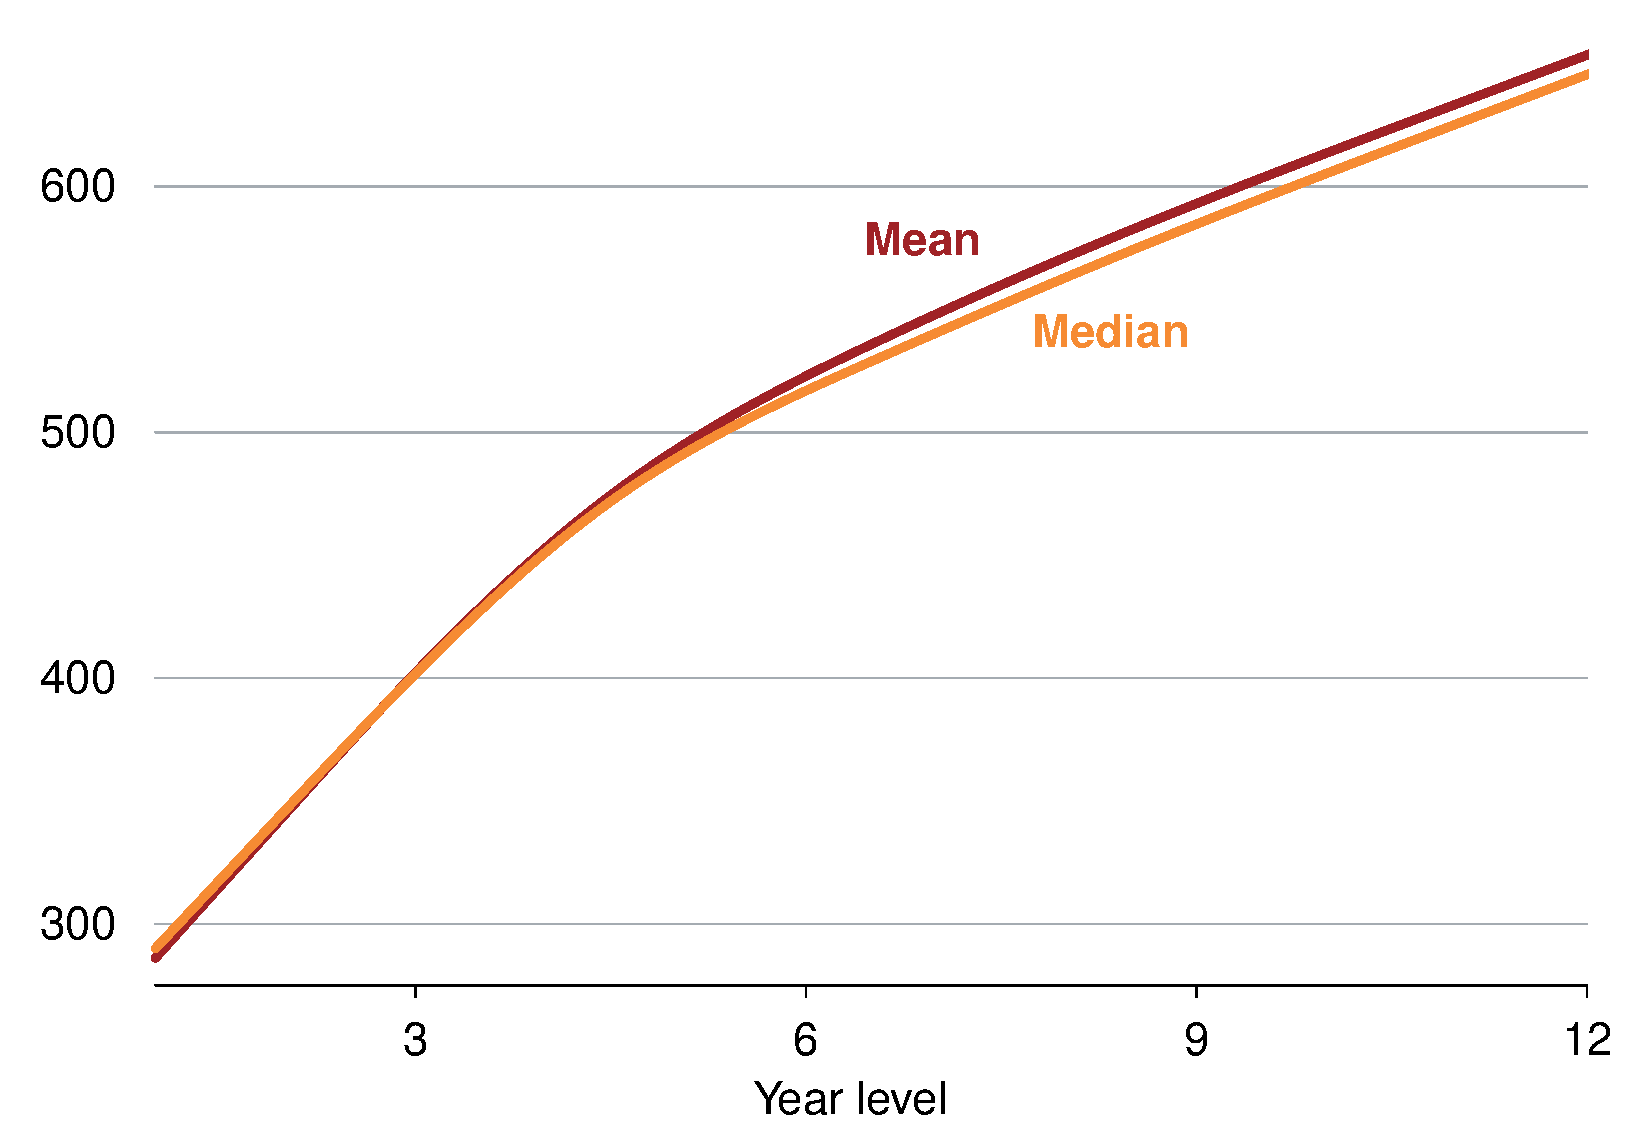
\includegraphics[width=\columnwidth]{atlas/mean_cyl.pdf}\label{fig:mean_cyl}

\source{Grattan analysis of \textcite{acara2014}.}
\end{figure}

Alternatively, instead of using a measure of central tendency such as the mean or median, the benchmark could be set much higher -- say, at the 80th percentile. A \textit{year of progress} would then be something harder for students to attain, but could be seen as something to aspire to. A curve based on the 80th percentile would be a better way of grouping high achieving students (for instance, those with NAPLAN scale scores above 650 in \mbox{Year 9}), but it would be difficult to accurately estimate what the 80th percentile student would have scored on a NAPLAN test taken before \mbox{Year 3}. Thus, this curve is unlikely to provide a good measure of progress over six years for average and below-average students.

In any case, it is worth noting that all percentiles between the 10th and the 90th appear to be concave, as shown in \Vref{fig:percentiles}. This suggests that the key findings of the report -- such as the gaps in student progress between different sub-groups -- would still hold even if equivalent year levels were estimated for a different percentile.

\begin{figure}[t]
 \captionwithunits{All percentiles make smaller gain scores at higher year levels}{NAPLAN scale score by percentile, numeracy, Australia}
 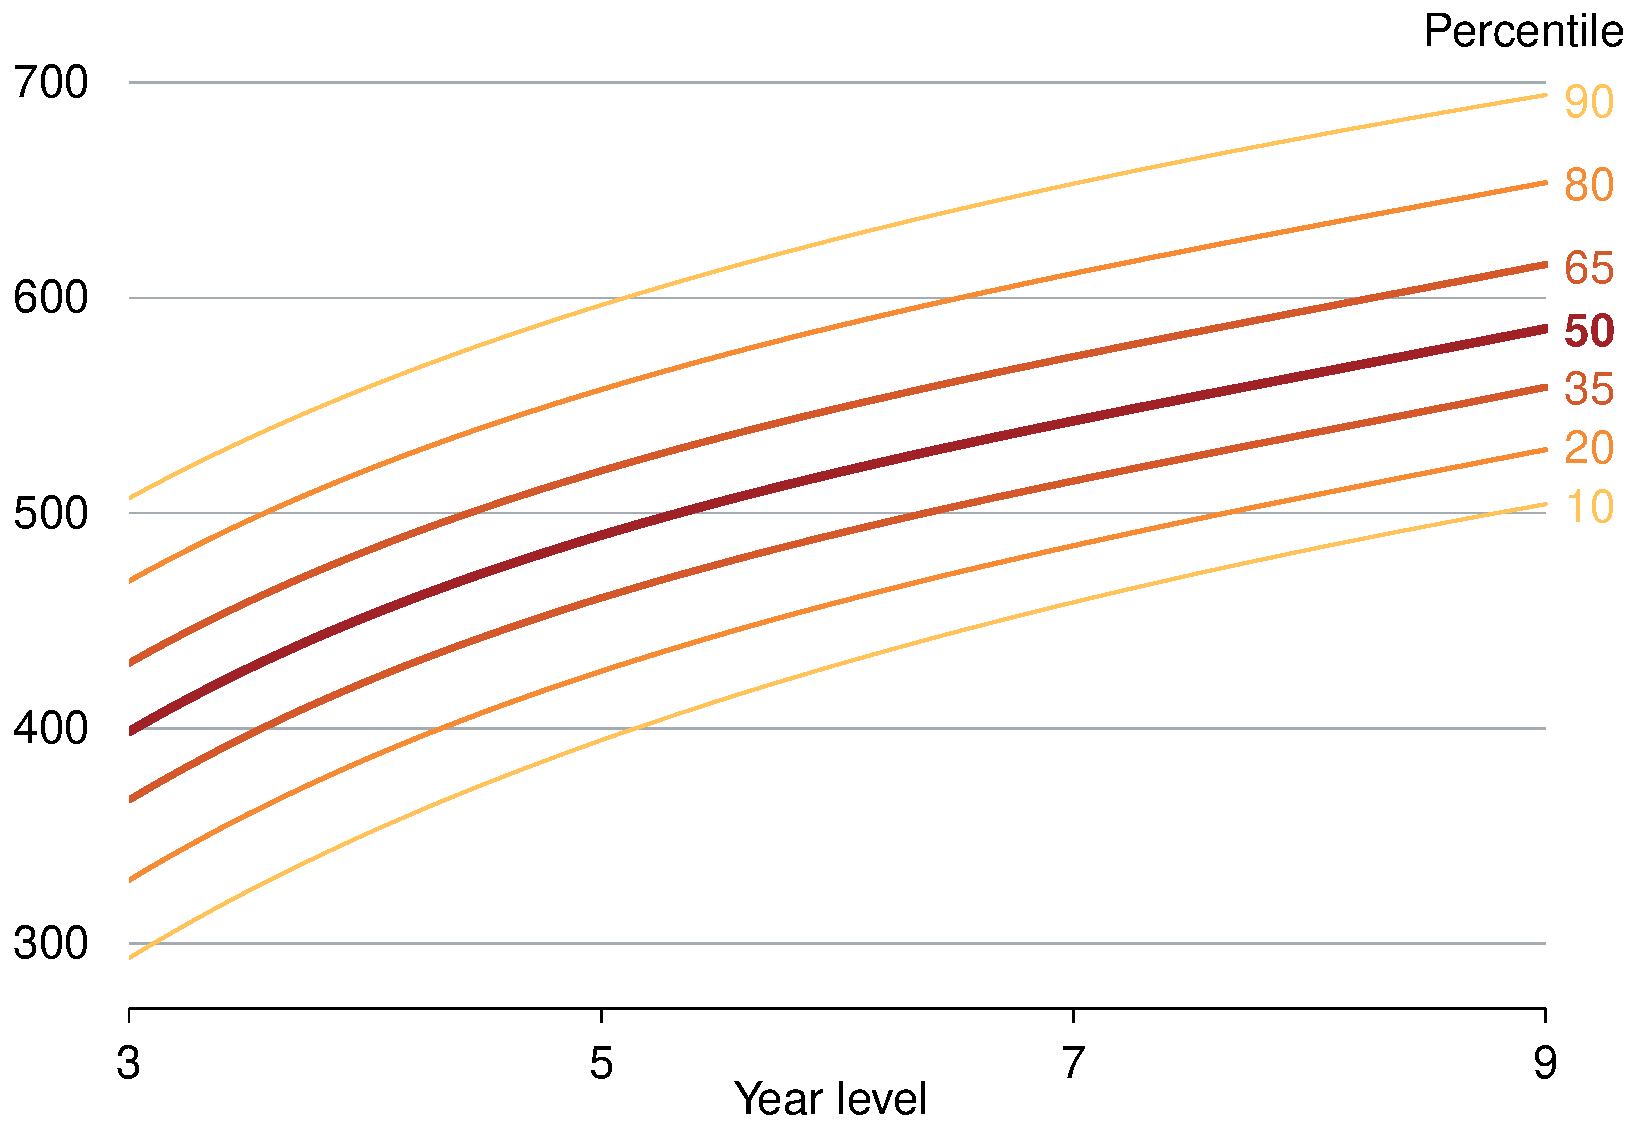
\includegraphics[width=\columnwidth]{atlas/Percentiles_N.pdf}\label{fig:percentiles}
 \notes{Percentiles defined according to 2014. Each curve is smoothed across four observed points using a third-order polynomial to get a better picture of the relationship. A similar pattern occurs for reading.}

\source{Grattan analysis of \textcite{acara2014}.}
\end{figure}

\subsubsection{Using control variables to estimate gain scores}

One assumption that was strongly considered in this methodology was to include control variables in \cref{eq:g_jY} -- the equation for $g_{j,Y}$. The rationale behind this is that $\widehat{g}_{j,5}$ is estimated for below-average students, and $\widehat{g}_{j,9}$ is estimated for above-average students, even though both are used as a proxy for the median student. Including control variables such as parental education and occupation could allow us to adjust for the non-representativeness of the sample of above-average or below-average students.

\newpage
This approach results in an benchmark curve that is steeper for lower scores, and flatter for higher scores. While using control variables makes intuitive sense, when $g_{j,Y}$ is estimated without control variables, our estimated equivalent year levels will provide more conservative estimates of the gaps in student progress between different sub-groups. We felt it was better to go with a more conservative approach.\footnote{In addition to being less conservative, using control variables may exacerbate the impact of regression to the mean, potentially introducing more error into the analysis.}

\subsubsection{Treatment of missing data}

Students that are exempt, absent, or withdrawn from a NAPLAN test in either 2012 or 2014 are ignored for the purposes of estimating the median NAPLAN scale score in each year level. But Section \ref{sec:missing} suggests that students who miss a test are more likely to come from households with lower parental education, and are likely to make smaller gain scores from a given prior score than other students. This means the estimated median score is likely to be above the true 50th percentile.

An alternative approach would assume that all students who missed a test would have scored below the median had they taken the test. Obviously some students that missed a test would score above the median, but it is likely that a significant majority of students who missed a test would have been below average. Thus, treating missing data as below the median may better approximate the median score than ignoring missing data.

\Cref{fig:missing_median} shows that this alternative treatment of missing data will, unsurprisingly, lead to a lower estimate of the median NAPLAN scale score in each year level. But the curves for both reading and numeracy still have the same concave shape. It is unlikely that this alternative treatment of missing data would lead to very different conclusions about the gaps in student progress. 

\begin{figure}[H]
 \captionwithunits{Treating missing data as below the median does not change the shape of the curve}{Estimated median NAPLAN scale score, Australia}

 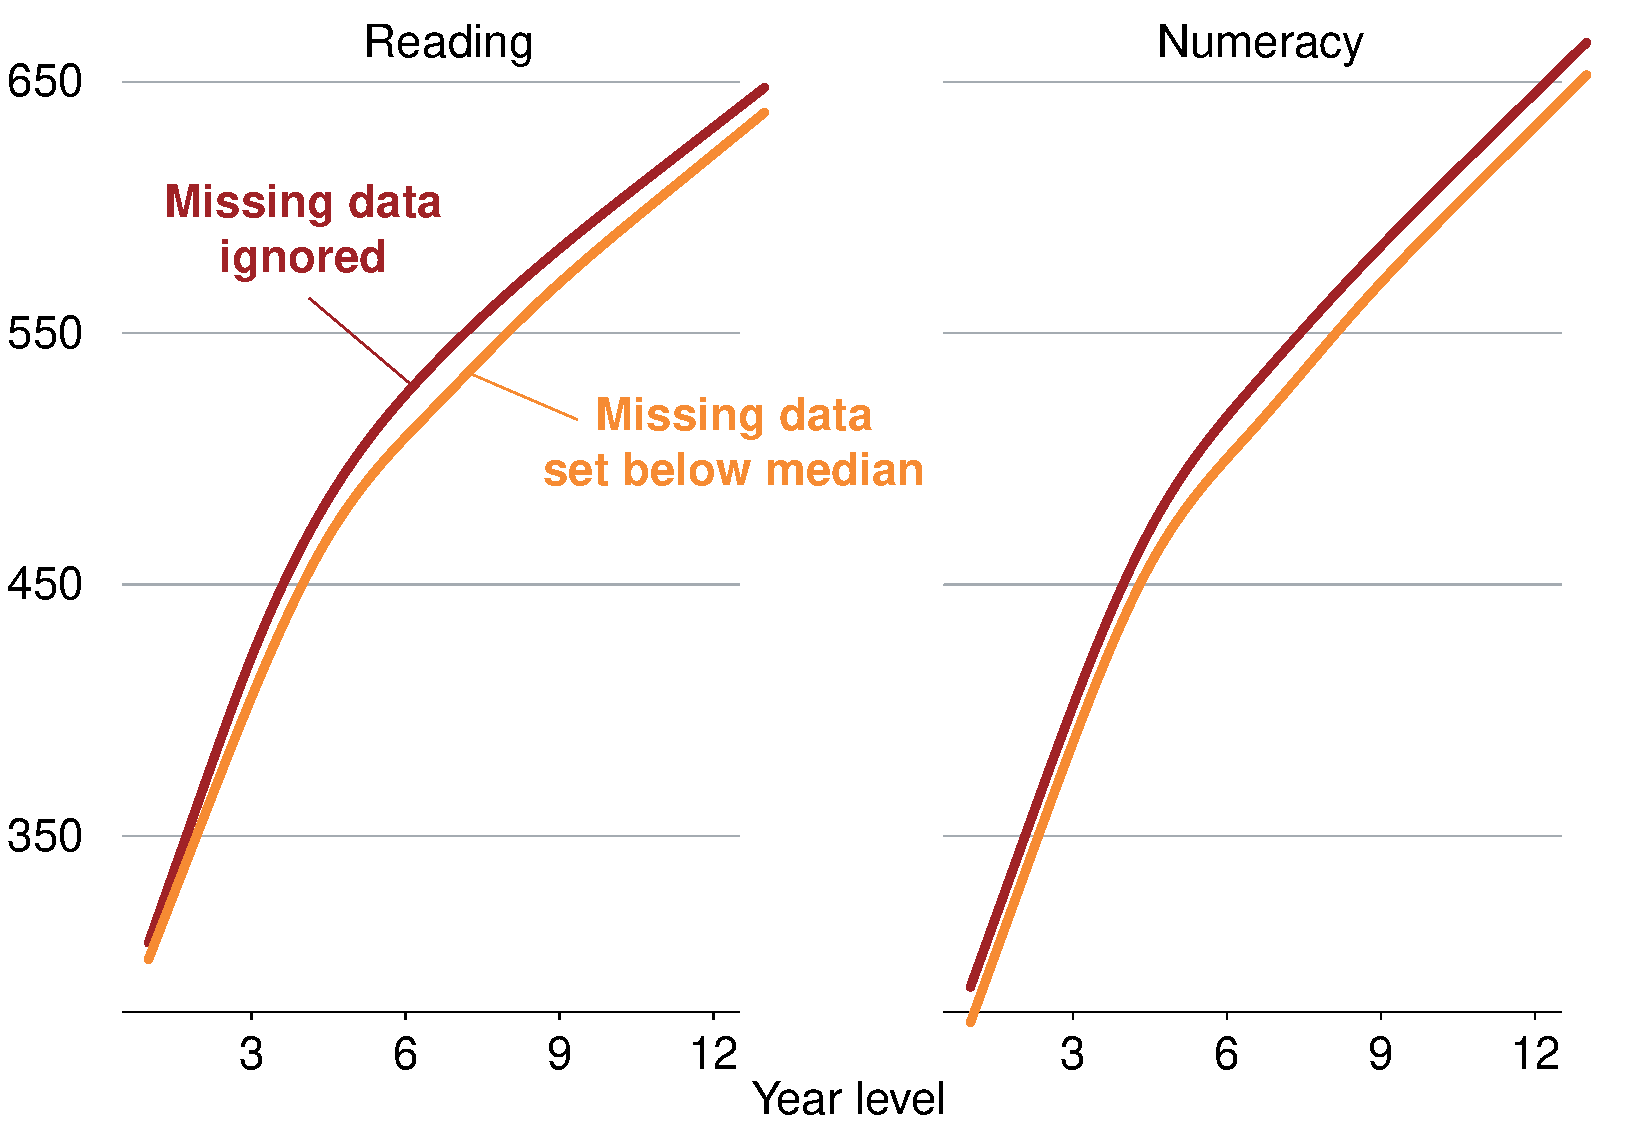
\includegraphics[width=\columnwidth]{atlas/missing_median.pdf}\label{fig:missing_median}

\source{Grattan analysis of \textcite{acara2014}.}
\end{figure}
\vspace{-15pt}

\subsection{How robust are estimates to different cohorts} \label{sec:cohort1}

It is not uncommon for the distribution of NAPLAN results to change across different cohorts. This could be due to improvements or changes in the way that certain subjects are taught, or differences in the characteristics of two cohorts.\footnote{For example, Queensland introduced a Prep school year in 2008, meaning that the cohort of \mbox{Year 5} students in 2013 are older than the cohort of \mbox{Year 5} students in 2012.} At the national level, results are not expected to change significantly across two cohorts one year apart.

We cross-checked our results by applying the methodology to the national cohort of 2013 students, with results linked to 2011. As \Cref{fig:cyl_2013} shows, in reading, the 2011-13 results are almost identical to those of 2012-14, except for Year 1 where the standard error is high (see Section \ref{sec:se_pe}). In numeracy, there is little noticeable difference below \mbox{Year 9}, but the estimated curve using the 2011-13 data is flatter for later year levels. This means the 2012-14 numeracy curve will provide more conservative estimates of progress for high achievers, students with high levels of parental education and students from high advantaged schools. 

\begin{figure}[t]
 \captionwithunits{There are some discrepancies that arise with different cohorts}{Estimated median NAPLAN scale score, Australia}
% \vspace{-1.2em}
 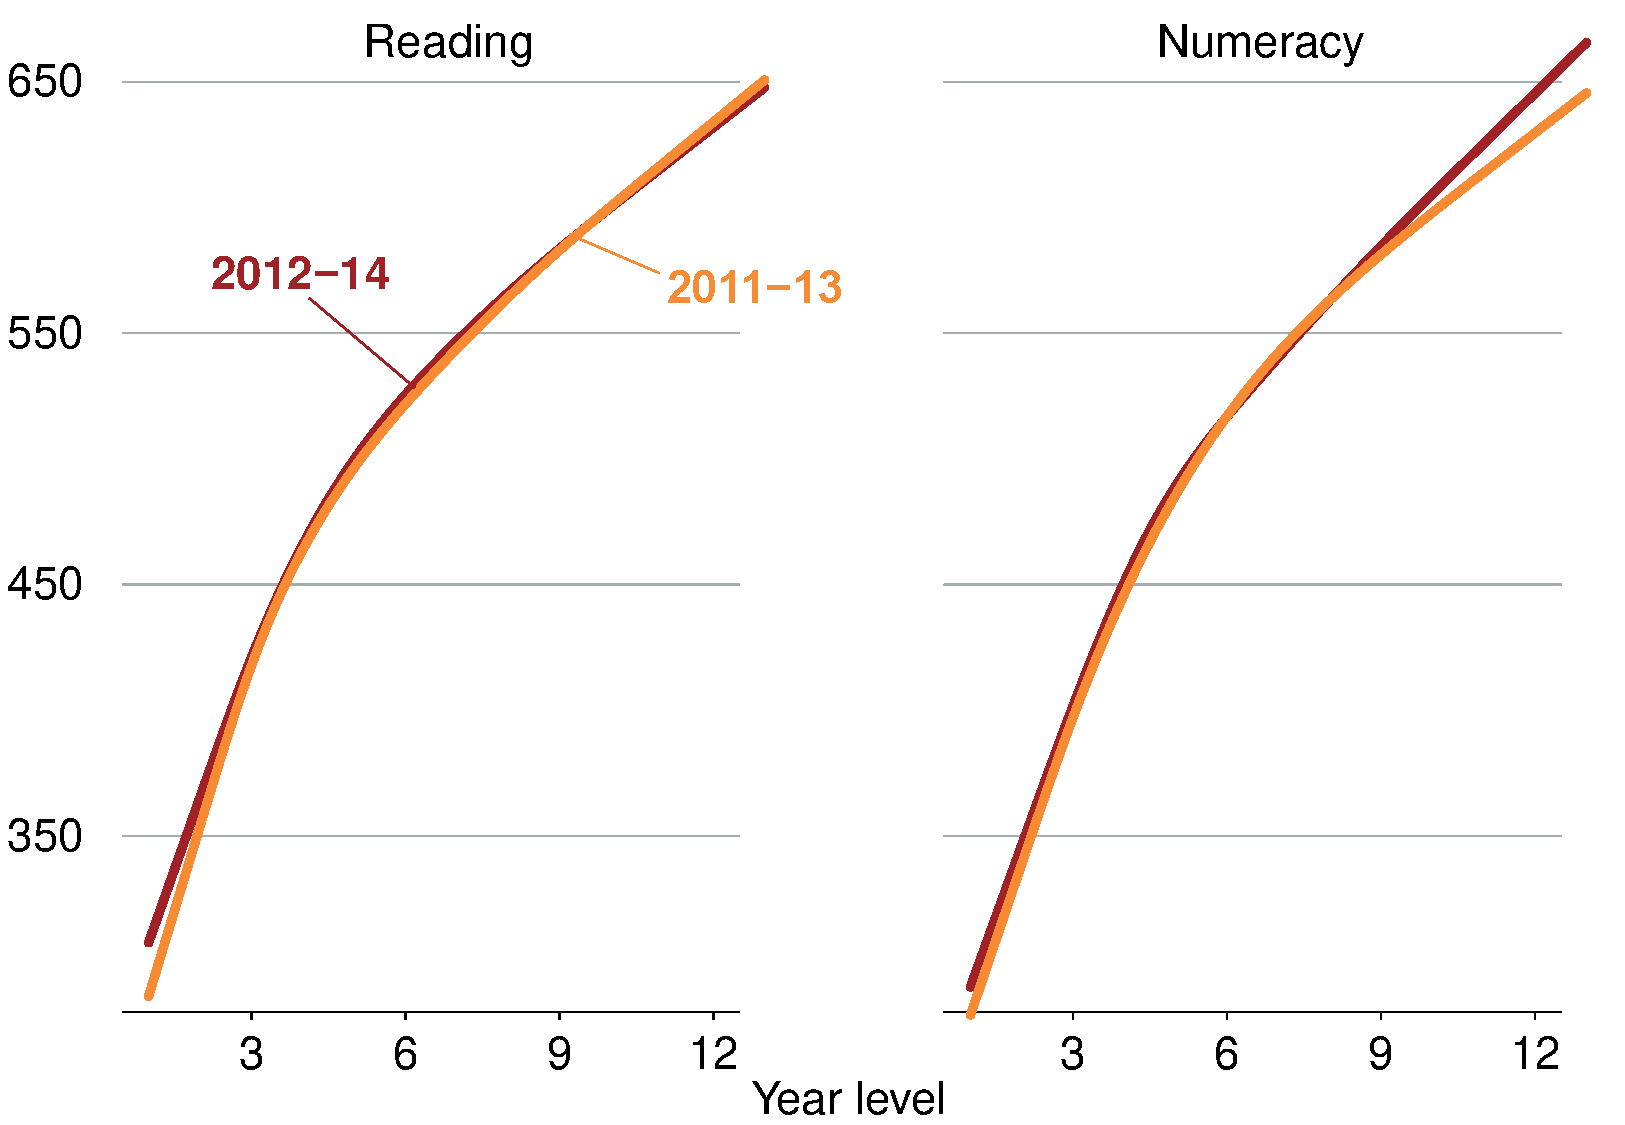
\includegraphics[width=\columnwidth]{atlas/cyl_2013.pdf}\label{fig:cyl_2013}

\source{Grattan analysis of \textcite{acara2013,acara2014}.}
\end{figure}

\newpage
\section{How equivalent year levels could be implemented as part of NAPLAN reporting}

Reporting NAPLAN results in terms of equivalent year levels provides a new interpretation of how students are learning relative to their peers. Given the importance of measuring student progress, and the limitations of NAPLAN gain scores, we believe this is an important contribution that should be considered as part of the official reporting of NAPLAN results by state education departments.

Of course, it is also important to consider the limitations of this approach. In terms of the methodology outlined in this chapter, equivalent year levels are not an appropriate way of reporting individual student results. This is because equivalent year levels do not cover the full range of NAPLAN scale scores, so this measure is inappropriate for high-achieving students (those performing above equivalent year level 12). In addition, high levels of measurement error at the individual level mean that it is difficult to accurately assign a student to an equivalent year level.\footnote{For a student above \mbox{Year 9} standard, their standard error could easily exceed one equivalent year level.}

\newpage
These issues are mitigated somewhat at the school level, provided that there are a sufficient number of students to reduce measurement error, and that most students perform below \mbox{Year 12} level. It should be possible to estimate an equivalent year level curve that adjusts for school background factors, but this is beyond the scope of this report. In any case, the greatest value of our approach is in measuring the progress of different cohorts and sub-groups with a common benchmark.

If this approach was to be implemented as part of NAPLAN reporting, there are a number of approaches that may improve the accuracy of the measure. First, the move to NAPLAN online will strengthen the vertical and horizontal equating process, thereby improving the accuracy of equivalent year levels. Second, it would be useful to sample students outside the NAPLAN test-taking years to validate the estimates of the median score in these years. For instance, if a NAPLAN test was given to a small number of students in \mbox{Year 2} and \mbox{Year 10}, this would lead to more accurate estimates of performance in these year levels. Finally, the curve could be estimated as the average of multiple cohorts to reduce the discrepancies between cohorts. 








